\section{Hardware}
Hier erwähnen was Platine alles für Aufgaben hat
Um die Segel des Windkraftwerkes jederzeit für maximale Effizienz eingestellt zu haben, müssen diese dynamisch Eingestellt werden können. Hierfür überwacht ein Controllino, die über Sensoren seine Umgebung und berechnet daraus die optimale Segel Einstellung. (KP sollte besser schon früher erwähnt werden/bzw wurde eventuell schon erwähnt)
\subsection{Vorgehen}
Bei dem Entwurf der Hardware sind mehrere Dinge zu beachten. Da das Sailwind 4.0 Projekt noch in den Startschuhen steht, sind einige dieser Faktoren auch noch nicht klar Bestimmbar zum Zeitpunkt dieser Arbeit. Aus diesem Grund wurden an manchen Stellen die Design Kriterien freier oder unnötig Komplex ausgelegt.\\

Um die Steuerung der Segel zu ermöglichen wird ein System benötigt das alle nötigen Akteure und Sensoren, Ansteuret und Überwacht. Hierfür soll eine Steuerelektronik Hardware entworfen werden. Da sich diese im Außeneinsatz befindet sollte diese in einem Wasserdichten Gehäuse eingeschlossen sein. Eine vorrausgehende Gruppe hatte bereits die Steuerelektronik entworfen, diese war allerdings zu groß dimensioniert und hatte einige Fehler, weswegen ebenfalls ein kleinere Formfaktor und die Behebung der Probleme als Ziel gesetzt wurden. Die Steuerelektronik soll Manuell Bedienbar sein, wewegen am Gehäuse ebenfalls eine Bedienmöglichkeit existieren sollte.

\label{Analyze_der_Aktoren_und_Sensoren}
\subsection{Analyze der bestehenden Hardware Elemente}
Um eine geeignete Steuerplatine zu entwerfen, bedarf es einer Analyze der anzusteurenden Hardware Komponenten. Diese wurden bereits vorrausgehend festgelegt und wurden übernommen. Diese können in die Kategorien Sensoren und Aktoren gruppiert werden. Dabei wurden die benötigte Spannung, der Stromverbrauch und die Schnittstellen betrachtet. Durch die Spannung und die Stromaufnahme kann später die benötigte Spurenbreite auf der Platine bestimmt werden. Die Schnittstellen geben an wie mit dem jeweiligen Gerät kommuniziert werden kann und welche davon benötigt werden.\\

\subsubsection{Sensoren}
Zu den Sensoren zählen die folgenden Komponenten:
\begin{itemize}
	\item Induktiver Endschalter: IFM IFS204
	\item Optischer Abstandssensor: IFM OGD580
	\item Anemometer: MESA WSWD
	\item Druckkraft-Sensor: Burster 8532
\end{itemize}

\noindent\textbf{Induktiver Endschalter}\newline
Zwei der IFM IFS204 Endschalter sind im Design mit eingebaut. Sie funktioneren als PNP-Schließkontakt und geben an einem Ausgang ein 24V high Signal aus, sobald sie ausgelöst werden. Dabei hat jeder Endschalter eine typische Stromaufnahme von <10mA und eine Betriebsspannung von 9-30V.\\

\noindent\textbf{Optischer Abstandssensor}\newline
Der Abstandssensor OGD580 funktioniert über einen Laser der vom Gerät ausgehend über eine reflektive Fläche zu diesem zrückgeworfen wird. Der Abstandsensor verfügt über ein Display das den gemessen Abstand anzeigt und über den das Gerät konfigurierbar ist. Er hat eine typische Stromaufnahme von ???mA und ebenfalls eine Betriebspannung von 9-30V. Der Abstand wird über einen Digitalen Ausgang, dem sog. IO-Link ausgegeben. Da dieser typischerweise nur in der Automobilbranche zum Einsatz kommt, wurde ein zusätzlicher IO-Link Konverter hinzugefügt. Der EIO104 konvertiert die digitale IO-Link Schnittstelle zu einer Analogen 4-20mA Schnittstelle mit der einfacher Umgegangen werden kann. Dabei kommt ein zusätzlicher Stromverbrauch von ???mA hinzu.\\

\noindent\textbf{Anemometer}\\
Das WSWD Anemometer wird genutzt um die Windrichtung als auch die Windgeschwindigkeit zu messen. Dieser basiert ebenfalls auf einer 24V Versorgungsspannung und hat je nach Konfiguration und Ausführung eine Stromaufnahme von 120mA. Er besitzt ebenfalls ein Heizelement um ihn bei sehr niedrigen Temperaturen nutzen zu können. Dieses wird allerdings im Einsatzszenario und im Prototyp nicht benötigt. Die Schnittstellen des Anenometers sind abhängig von dessen ausführung. In der zum Einsatzkommenden Ausführung, dem WSWD1, kann neben einer Analogen Schnittstelle die Daten auch über eine Digitale RS485/RS422 Schnittstelle abgefragt werden. Die Werte können Analog entweder als ein 0/4-20/24mA Signal oder als ein 0/2-8/10V Signal ausgegeben werden. Die Digitale Schnittstelle kann neben der Datenausgabe auch zur Konfiguration des Gerätes genutzt werden und bietet eine Vielzahl an Protokollen zur Kommunikation an.\\

\noindent\textbf{Druckkraft-Sensor}\newline
Der Burster Druckkraft-Sensor war der einzige Sensor der zum Zeitpunkt der Arbeit noch nicht Bestellt wurde. Dieser wurde aber dennoch mit eingeplant. Der Druckkraft Sensor kann ebenfalls mit den typischen 24V betrieben werden und hat dabei eine Stromaufnahme von ca. 12,5mA. Die Messwerte werden hier über eine Analoge 0-10V Schnittstelle übertragen.\\
\subsubsection{Aktoren}
Zu den Aktoren zählen die folgenden Komponenten:
\begin{itemize}
	\item Gleichstrommotor: Dunkermotoren BG 45x30 SI
	\item Externe Relais
\end{itemize}

\noindent\textbf{Gleichstrommotor}\newline
Der Dunkermotor BG 45x30 SI Gleichstrommotor ist das Kernelement des Aufbaus. Da der Motor eine interne Regelung besitzt hat er eine getrennte Leistungs- und Logikversorgung. Der Motor an sich wird dabei über den Leistungsteil bestromt, während über den Logikteil dieser gesteuert werden kann und Feedback bereitstellt. Die Betriebsspannung der Leistungs- und Logikversorgung sind 24V, wobei der Motor einen maximal zulässigen Dauerstrom von 3,8A ausgesetzt sein darf. Die Logikversorung hat eine Stromaufnahme von 100mA. Die Kommunikation mit dem Motor findet über vier Digitale- und einen Analogen Eingang statt. Der Motor stellt Feedback zum aktuellen Status über drei Ausgänge bereit. Diese geben die Drehrichtung, aktuelle Störungen und die Drehgeschwindigkeit des Motors an.\\
% Please add the following required packages to your document preamble:
% \usepackage{graphicx}
\begin{table}[H]
	\centering
		\begin{tabular}{|c|c|c|}
			\hline
			\textbf{Eingang 1 (IN1)} & \textbf{Eingang 0 (IN0)} & \textbf{Funktion}      \\ \hline
			0                        & 0                        & Motor aus              \\ \hline
			0                        & 1                        & Linkslauf              \\ \hline
			1                        & 0                        & Rechtslauf             \\ \hline
			1                        & 1                        & Stopp mit Haltemoment  \\ \hline
			\textbf{Eingang 3 (IN3)} & \textbf{Eingang 2 (IN2)} &                        \\ \hline
			0                        & 0                        & Drehzahlvorgabe Analog \\ \hline
			0                        & 1                        & Stromvorgabe Analog    \\ \hline
			1                        & 0                        & Geschwindigkeit 1      \\ \hline
			1                        & 1                        & Geschwindigkeit 2      \\ \hline
		\end{tabular}%
	\caption{Eingänge und Funktionen des BG 45x30 SI}
	\label{tab:digitale_Eingaenge}
\end{table}
Hier oder später noch Ein und Ausgänge definieren in Tabelle bzw. in Text erwähnen
\\

\noindent\textbf{Externe Relais}\newline
Zum Zeitpunkt der Arbeit gab es noch keinen konkreten Verwendungszweck der externen relais diese wurden für zusätzliche Funktionalitäten dennoch mit eingeplant und sollten über ein 24V Signal geschalten werden.\\

\noindent\textbf{Controllino}\newline
Der Controllino ist der zentrale Microcontroller und verwaltet alle Aktoren im System. Über diesen soll das hier zu entwerfende System, seine Befehle zur Segelausrichtung bekommen. Der Datenaustausch soll hier über eine Ethernet Schnittstelle stattfinden, um die Große Distanz zwischen Kuppel und Basis zu überbrücken.

\subsubsection{Zusammenfassung und Übersicht}
Damit sind nun alle externen anzusteurenden Komponenten abgedeckt. Die benötigte Stromversorgung sowie alle Schnittstellen sind dabei in \autoref{tab:uebersicht-externe-elemente} dargestellt. Dabei kann bereits entnommen werden, das es sehr sinnvoll ist die Platine auf ein 24V System auszulegen und diese auch mit dieser Spannung zu versorgen.
% Please add the following required packages to your document preamble:
% \usepackage{graphicx}
\begin{table}[H]
	\centering
	\resizebox{\textwidth}{!}{%
		\begin{tabular}{|l|lllllllllll|}
			\hline
			\textbf{Element} & \multicolumn{11}{l|}{\textbf{Pinout}} \\ \hline
			\textbf{Endschalter 1} & \multicolumn{1}{l|}{24V} & \multicolumn{1}{l|}{GND} & \multicolumn{1}{l|}{OUT} & \multicolumn{8}{l|}{} \\ \hline
			\textbf{Endschalter 2} & \multicolumn{1}{l|}{24V} & \multicolumn{1}{l|}{GND} & \multicolumn{1}{l|}{OUT} & \multicolumn{8}{l|}{} \\ \hline
			\textbf{Abstandssensor} & \multicolumn{1}{l|}{24V} & \multicolumn{1}{l|}{GND} & \multicolumn{1}{l|}{IO-Link} & \multicolumn{8}{l|}{} \\ \hline
			\textbf{IO-Link Konveter} & \multicolumn{1}{l|}{24V} & \multicolumn{1}{l|}{GND} & \multicolumn{1}{l|}{AOUT} & \multicolumn{8}{l|}{} \\ \hline
			\textbf{Anemometer} & \multicolumn{1}{l|}{24V} & \multicolumn{1}{l|}{GND} & \multicolumn{1}{l|}{AOUT} & \multicolumn{1}{l|}{AOUT} & \multicolumn{1}{l|}{AGND} & \multicolumn{1}{l|}{RS485+} & \multicolumn{1}{l|}{RS485-} & \multicolumn{4}{l|}{} \\ \hline
			\textbf{Druckkraftsensor} & \multicolumn{1}{l|}{24V} & \multicolumn{1}{l|}{GND} & \multicolumn{1}{l|}{AOUT} & \multicolumn{1}{l|}{AGND} & \multicolumn{7}{l|}{} \\ \hline
			\textbf{Motor Leistung} & \multicolumn{1}{l|}{24V} & \multicolumn{1}{l|}{GND} & \multicolumn{9}{l|}{} \\ \hline
			\textbf{Motor Logik} & \multicolumn{1}{l|}{24V} & \multicolumn{1}{l|}{GND} & \multicolumn{1}{l|}{IN0} & \multicolumn{1}{l|}{IN1} & \multicolumn{1}{l|}{IN2} & \multicolumn{1}{l|}{IN3} & \multicolumn{1}{l|}{AIN} & \multicolumn{1}{l|}{AGND} & \multicolumn{1}{l|}{OUT1} & \multicolumn{1}{l|}{OUT2} & OUT3 \\ \hline
			\textbf{Externes Relais 1} & \multicolumn{1}{l|}{OUT} & \multicolumn{1}{l|}{GND} & \multicolumn{9}{l|}{} \\ \hline
			\textbf{Externes Relais 2} & \multicolumn{1}{l|}{OUT} & \multicolumn{1}{l|}{GND} & \multicolumn{9}{l|}{} \\
			\hline
			\textbf{Controllino} & \multicolumn{1}{l|}{Ethernet} & \multicolumn{10}{l|}{} \\ \hline
		\end{tabular}%
	}
	\caption{Übersicht Stromversorgung und Schnittstellen der externen Elemente}
	\label{tab:uebersicht-externe-elemente}
\end{table}
\subsection{Auswahl der Platinen Bauteile}
Da nun klar ist welche Anforderungen durch die anzuschließenden Geräte bestehen, kann auf Basis dieser nun weiterverfahren werden. Dabei soll im folgenden ein geeigneter Mikrocontroller, sowie die nötigen Platinenkomponenten ausgewählt werden, um mit den Hardwarekomponenten zu kommunizieren und diese mit Strom zu versorgen.
\subsubsection{Mikrocontroller}
Die Auswahl des Mikrocontrollers wurde auf der Basis folgender Kriterien beschlossen:
\begin{itemize}
	\item Anzahl Inputs und Outputs
	\item Architektur
	\item Softwaresupport
	\item Entwicklung
	\item Verfügbarkeit
\end{itemize}
Dabei gab es die Option den Chip als einzelnes Element direkt auf die selbst erstellte Platine einzubetten oder ein Entwicklungsboard als Basis zu nutzen und eine Erweiterungsplatine dafür zu nutzen. Es wurde sich dabei für ein Entwicklungsboard entschieden um bereits parallel zum Hardwaredesign eine geeignete Software zu entwickeln und diese bereits mit einem Prototypischen Aufbau zu testen (Vielleicht noch erwähnen, probleme bei vorheriger Gruppe). Dies bietet ebenfalls den Vorteil, das bei fatalen Fehlern ein schneller Ersatz angebracht werden kann und auch bereits ein Formfaktor vorgegeben ist.\\

Durch die große Anzahl an benötigten Inputs und Outputs und den relativ großen Anspruch an Onboard Speicher z.B für den geplanten Webserver, wurde sich für eine 32Bit Architektur entschieden.
\subsubsection{Relais}
Um das Endschalter Ausgangssignal an den Mikrocontroller weiterzugeben, werden zwei 24V Relais genutzt die bei der Aktivierung der Spule ein 3,3V Signal an den Eingang des Mikrocontrollers weitergeben. Gleichzeitig wird durch das Umschalten des Relais der Eingang 1 oder 2 auf Null gesetzt, so das dieser direkt Ausgeschaltet wird um eine Kollision mit den Enden der Linearführung vorzubeugen.
\subsubsection{Optokoppler}
Um die restlichen 24V Aus- und Eingänge zu steueren oder auszulesen kommen Optokoppler zum Einsatz. Diese isolieren ähnlich zu Relais den 24V und 3,3V Schaltkreis und ermöglichen es durch einen kleinere Spannung eine größere Last zu schalten. Dabei werden insgesamt 9 benötigt um die digitalen Ein und Ausgänge des Motors und die beiden externen Relais zu schalten. Da es sich beim Ausgang 3? des Motors um ein Pulsierendes Signal zur Ermittelung der Drehgeschw. des Motors handelt wurde auf eine schnelle Schaltzeit der Optokoppler geachtet (hier Berechnung einfügen).
\subsubsection{RS485 zu UART Konverter}
Um das Anemometer über die RS485 Schnittstelle zu konfigurieren und Daten abzufragen wird ein zusätzlicher Baustein benötigt. Dieser Konvertiert das differenzielle RS485 Signal zu einem nicht differenziellen UART Signal, das der Microcontroller untertsützt.
\subsubsection{FRAM}
Da die mittlere Position des Segels eingestellt werden können soll, wird ein nicht flüchtiger Speicher benötigt in dem die Position gespeichert wird. Dabei ist der FRAM eine der billigsten Speichermöglichkeiten für diesen Zweck, dabei wurde die geringste Speichergröße gewählt, da dieser wie ein EEPROM jederzeit überschrieben werden kann.
\subsubsection{Operations Verstärker}
Um die Drehzahl des Motors vorgeben zu können, wird ein Analoges Signal im Bereich von 0-10V benötigt. Da der Mikrocontroller bei einer Versorgungsspannung von 5V maximal ein Analoges Signal von 5V Ausgeben kann, wird ein Operationsverstärker benötigt. Dieser soll mit der 24V Versorgungsspannung das 0-5V Signal verstärken und auf die 0-10V skalieren.
\subsubsection{Spannungsregler}
Um alle Komponenten zu versorgen Bedarf es insgesamt 3 verschieden Spannungspotenzialen: 24V, 5V und 3,3V. Um dies zu erreichen sollen alle externen Elemente direkt mit den 24V versorgt werden. Der Mikrocontroller soll mit den 5V versorgt werden, da er somit auch ohne Debugger Erweiterung genutzt werden kann. Hierfür wird ein Step Down konverter genutzt der die 24V Versorgungsspannung auf 5V herunterbricht. mit diesen 5V kann daraufhin ein Festspannungsregler betrieben werden der die 5V auf eine 3,3V Spannung herunter bringt mit einem sehr geringen ripple.
\subsubsection{Platinen Entwurf}
Hier Schaltplan und Gerendertes Bild einfügen
\subsubsection{Analoge Eingänge}
Um die Analogen Ausgänge des Abstandsensors und des Anemometers auszulesen wird das 4-20mA Stromsignal über einen Widerstand zu einem 0-3V Spannungssignal gewandelt das mit dem \ac{ADC} des Microcontrollers gelesen werden kann.
Spannungsteiler
Strom zu Spannung
Widerstände
\subsection{Gehäuse und Anschlüsse}
Hier Freecad Bild einfügen für mount und Gehäuse
\subsection{\ac{HMI}}
Das HMI besteht aus einer Reihe von Kippschaltern, Knöpfen und LEDs. Diese sind sind in \autoref{fig:Bedienung} dargestellt. Dabei soll die gewünschte Neutrale Position der Linearführung durch einen Manuellen Betrieb stattfinden. Dabei kann der Endnutzer über die Trimm und Roll Knöpfe zum gewünschten Mittelpunkt Navigieren und diesen mit dem dritten Knopf speichern. Anschließend kann mittels des Kippschalters in den Automatik Betrieb gewechselt werden in dem das betätigen der Knöpfe ignoriert wird.
Eine Reihe von LEDs gibt Feedback über den aktuellen Zustand der Linearführung. Dabei wird konstant der aktuelle Betriebsmodus durch zwei LEDs angegeben. Ebenfalls wird die Position relativ zur festgelegten neutral Position durch zwei gelbe LEDs angegeben. Eine Störung in der Steuerung oder im Motor wird durch eine rote LED angegeben.\\
Die Knöpfe und Kippschalter sind beide am Gehäuse montiert und sind Spritzwasser geschützt. Im Gegensatz dazu sind die LEDs direkt auf der Platine platziert und werden durch flexible Lichtleiter zur Außenseite des Gehäuses geführt.
\begin{figure}[H]
	\centering
	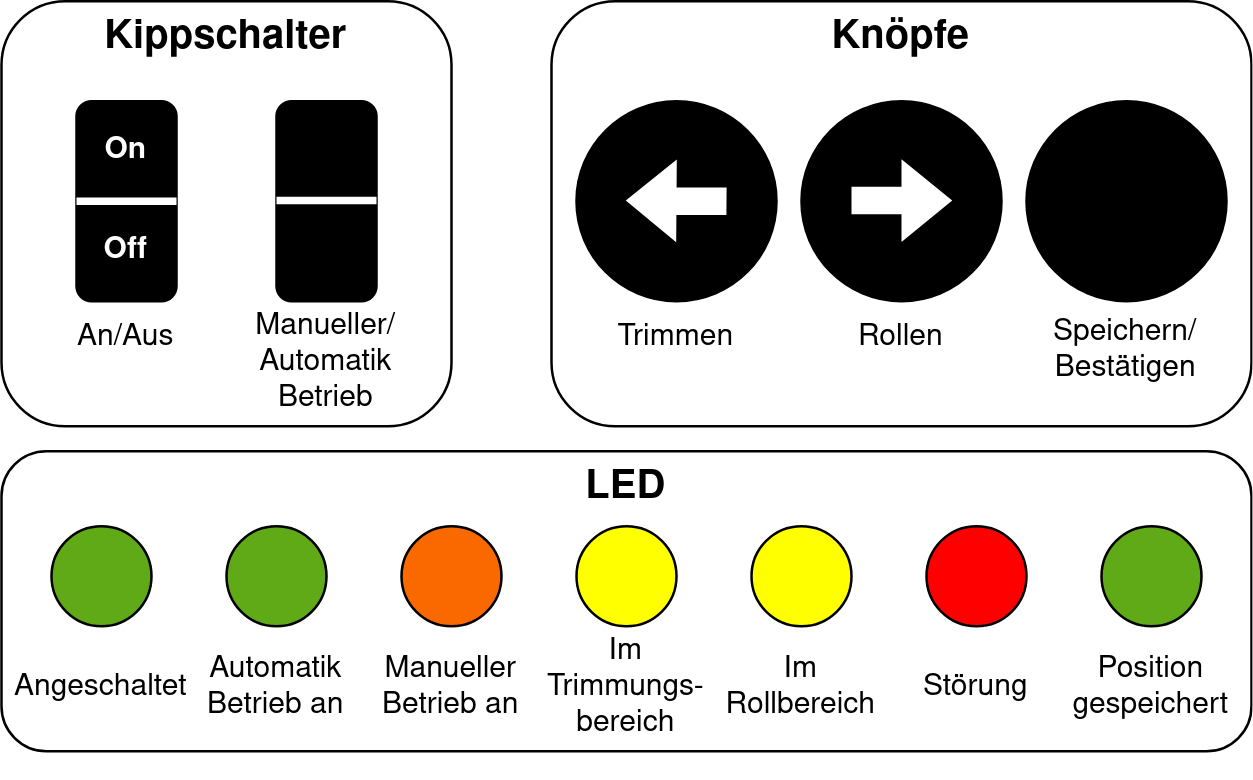
\includegraphics[width=1.0\textwidth]{images/Hardware/Bedienung.drawio.png}
	\caption{HMI der Segel Steuerung}
	\label{fig:Bedienung}
\end{figure}

\subsection{Probleme}
Klemmenlöcher
Operationsverstärker
Widerstände RS485
FRAM MOSI/MISO